\documentclass{article}

\usepackage[utf8]{inputenc}
\usepackage[T1]{fontenc}

\usepackage{tikz-er2}
\usetikzlibrary{positioning}
\usetikzlibrary{shadows}

\usepackage{subcaption}
\usepackage{enumitem}
\usepackage{hyperref}
\usepackage{ulem}



\begin{document}
\title{Chess Openings Database Specification}
\author{Yoan Geran \and Colin Geniet}
\maketitle

\tableofcontents

\section{Relational schema}
As a reminder, the EER schema from the first part is in figure \ref{eer}.
The translated relational schema is in figure \ref{db}.


\tikzstyle{every entity} = [top color=white, bottom color=blue!30, 
                            draw=blue!50!black!100, drop shadow]
\tikzstyle{every weak entity} = [drop shadow={shadow xshift=.7ex, 
                                 shadow yshift=-.7ex}]
\tikzstyle{every attribute} = [top color=white, bottom color=yellow!20, 
                               draw=yellow, node distance=1cm, drop shadow]
\tikzstyle{every relationship} = [top color=white, bottom color=red!20, 
                                  draw=red!50!black!100, drop shadow]
\begin{figure}
\caption{EER schema}
\label{eer}
\begin{center}
\scalebox{.80}{
\begin{tikzpicture}[every edge/.style={link}]
    \node[entity] (game) {Game};
    
    \node[relationship] (white) [below right= 0cm and 1cm of game] {white} edge node [auto] {1} (game);
    \node[relationship] (black) [above right= 0cm and 1cm of game] {black} edge node [auto,swap] {1} (game);
    \node[entity] (player) [above right= 0cm and 1cm of white] {Player} edge (white);
    \draw[link] (player) edge (black);
    
    \node[relationship] (gevent) [above left= 1cm and 0cm of game] {in event} edge node [auto] {1} (game);
    \node[entity] (event) [left= 0.5cm of gevent] {Event} edge (gevent);
    
    \node[relationship] (gopening) [left= 5cm of game] {\sout{played in}} edge (game);
    \node[entity] (opening) [above= 1cm of gopening] {Opening} edge (gopening);
    \node[relationship] (variation) [above= 0.5cm of opening] {\sout{variation}};
    \draw[link] (opening.70) edge (variation.283);
    \draw[link] (opening.110) edge (variation.257);
    
    \node[draw,circle,top color=white, bottom color=green!20, draw=green!50!black!100, drop shadow] (obj_is) 
         [above= 6cm of game] {D} edge (game) edge (opening) edge (event) edge (player);
    \node[entity] (object) [above= 1cm of obj_is] {Object} edge node {$\bigcup$} (obj_is);
    
    \node[relationship] (owns) [left= of object] {owns} edge [total] node [auto] {1} (object);
    \node[entity] (user) [left= of owns] {User} edge (owns);
    \node[relationship] (edit) [below left= 1cm and 1.2cm of object] {can edit} edge [total] (object) edge (user);
    
    \node[relationship] (on) [above= 1cm of object] {on} edge (object);
    \node[entity] (comment) [left= of on] {Comment} edge [total] node [auto] {1} (on);
    \node[relationship] (from) [above= 0.8cm of user] {from} edge (user) edge [total] node [auto] {1} (comment);
\end{tikzpicture}
}
\end{center}
\end{figure}

\begin{figure}
\caption{Relational schema}
\label{db}
\begin{center}
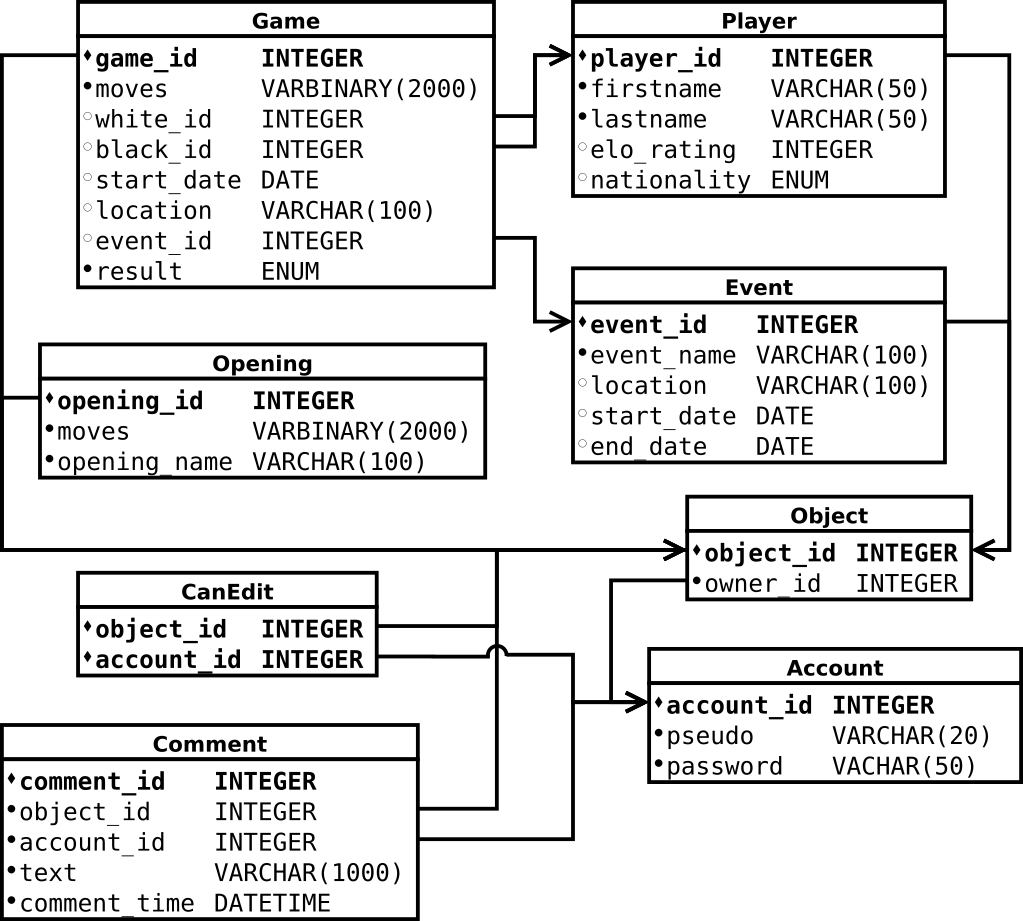
\includegraphics[scale=0.4]{relational}
\end{center}
Bold denotes primary keys, black and white dots denotes required and optional attributes respectively.
\end{figure}


\subsection{Change to EER model}
A change made to the entity relationship model during translation was the removal of the \verb|played in|
and \verb|variation| relations. The reason is that those two relationships could be --- 
as described in previous integrity constraints --- entirely defined as function of the \verb|moves| attributes 
of entities \verb|Game| and \verb|Opening|, and thus were entirely redundant.

We may re-add those tables during implementation for performance purpose, as search based on them is
a main part of this database system. The question of whether or not it is actually an interesting
improvement will however be left for part 3.

Anyways, we did not consider appropriate to include this redundancy in the high-level model.

\subsection{General translation}
Most of the translation is straightforward.
Entities are translated into relations, 1 to N relationships are inlined as foreign key attributes of the entity with cardinality 1.
The remaining relationship with cardinality N to N (\verb|can_edit|) is translated in a separate table.

\subsection{Translation of inheritance}
The one non-obvious choice in translation is that of inheritance of the entity \verb|Object|.
The whole point of \verb|Object| is to have unique ids for all objects (games, openings, \dots),
to allow a unique foreign key to refer any object unambiguously, and without use of a type field.

This makes it unsuitable to have relations for subclasses only, as it would be impossible to
enforce the uniqueness of ids among all subclasses using key constraints only.

Only having a relation for the \verb|Object| superclass would also be highly inappropriate
as the subclasses are extremely different, resulting in many \verb|NULL| fields.

This is why we chose to keep a relation for both the superclass and the subclasses, with the \verb|Object| superclass
being mostly used to enforce the id uniqueness constraint.


\section{Data representation}
As a general note, \verb|VARCHAR| fields widths are approximate, and will be fine-tuned during implementation.

\subsection{Chess moves representation}
Our choices for moves representation did not change since part 1.

Obviously, chess moves will be a very important --- and big --- part of this database.
Thus, finding an efficient representation for them is important.
The one we settled for is to represent any of the 64 squares by a byte.
A move is represented by two bytes, and a sequence of moves by a bytes sequence.

While not human readable, this representation is quite compact, totally unambiguous,
has an unique representation for any given move, and has constant representation
size for a move.

All those advantages are important when searching in the database for games starting
with a given move sequence, as the search is simply a prefix lookup.

The other representation we considered are:
\begin{itemize}
\item Algebraic notation is the most standard, but has problems with ambiguity
(two valid strings can represent the same move), making search much more complicated.
Additionally, it uses more space, and it has non-constant representation size.

\item Representing the start and end squares in plain text mostly keeps the advantages
of our representation while being human readable. However, it do uses twice more space.
Since having a human readable internal representation is not very useful,
we ruled it out.
\end{itemize}


\paragraph{Detailed representation}
Chess board squares are numbered from left to right, and from bottom to top,
starting with 0. Thus, \verb|a1| is numbered as 0, \verb|a8| as 7, \verb|b1| as 8, \dots
The square number is directly encoded in the six lower end bits of a byte.

For promotions, the two remaining higher end bits of the end square are used to represent the piece promoted to,
encoded as Queen=0 (values in range 0--63), Knight=1 (64--127), Rook=2 (128--191), Bishop=3 (192--255).
For instance, a white pawn promoting on column \verb|a| will be represented as 6--7 for a queen promotion,
6--71 for a Knight promotion, 6--135 for a Rook promotion and 6--199 for Bishop promotion.

Note that castling is represented by the King move.


\subsection{Other data types}
The following attributes use non-obvious data representation.

\paragraph{Game result}
Game result is represented with an enumeration: 'white', 'black', 'draw', 'undefined'.
A game result may be undefined if the game was interrupted for instance, or is still ongoing.

\paragraph{Nationality}
For nationality attributes, we decided to use ISO 3166-1 encoding.
To avoid additional integrity constraint, we chose to use an enum type for all the country codes
to enforce valid codes.

The alternative choice would have been to use a fixed size character field.



\subsection{Integrity Constraints}
\begin{itemize}
\item \verb|moves| attributes in relations \verb|Game| and \verb|Opening| must represent
valid sequences of chess moves starting from the initial chess position.

\item \verb|result| attribute in relation \verb|Game| must represent the result given by the
\verb|moves| attributes.

\item An user can edit any object they owns.
\end{itemize}

\end{document}